% REV01 Tue 22 Jun 2021 19:18:38 WIB
% START Tue 04 May 2021 13:55:16 WIB

\chapter{A RIDDLE WITHOUT AN ANSWER}

Again Mr Mortimer Lightwood and Mr Eugene Wrayburn sat together in the
Temple. This evening, however, they were not together in the place of
business of the eminent solicitor, but in another dismal set of
chambers facing it on the same second-floor; on whose dungeon-like black
outer-door appeared the legend:

\begin{center}
		\textbf{PRIVATE}\\[2pt]

		\textbf{MR EUGENE WRAYBURN}\\[2pt]

		\textbf{MR MORTIMER LIGHTWOOD}\\[2pt]

		\textbf{(Mr Lightwood’s Offices opposite.)}\\[2pt]
\end{center}

Appearances indicated that this establishment was a very recent
institution. The white letters of the inscription were extremely white
and extremely strong to the sense of smell, the complexion of the
tables and chairs was (like Lady Tippins’s) a little too blooming to
be believed in, and the carpets and floorcloth seemed to rush at the
beholder’s face in the unusual prominency of their patterns. But the
Temple, accustomed to tone down both the still life and the human life
that has much to do with it, would soon get the better of all that.

‘Well!’ said Eugene, on one side of the fire, ‘I feel tolerably
comfortable. I hope the upholsterer may do the same.’

‘Why shouldn’t he?’ asked Lightwood, from the other side of the fire.

‘To be sure,’ pursued Eugene, reflecting, ‘he is not in the secret of
our pecuniary affairs, so perhaps he may be in an easy frame of mind.’

‘We shall pay him,’ said Mortimer.

‘Shall we, really?’ returned Eugene, indolently surprised. ‘You don’t
say so!’

‘I mean to pay him, Eugene, for my part,’ said Mortimer, in a slightly
injured tone.

‘Ah! I mean to pay him too,’ retorted Eugene. ‘But then I mean so much
that I--that I don’t mean.’

‘Don’t mean?’

‘So much that I only mean and shall always only mean and nothing more,
my dear Mortimer. It’s the same thing.’

His friend, lying back in his easy chair, watched him lying back in his
easy chair, as he stretched out his legs on the hearth-rug, and said,
with the amused look that Eugene Wrayburn could always awaken in him
without seeming to try or care:

‘Anyhow, your vagaries have increased the bill.’

‘Calls the domestic virtues vagaries!’ exclaimed Eugene, raising his
eyes to the ceiling.

‘This very complete little kitchen of ours,’ said Mortimer, ‘in which
nothing will ever be cooked--’

‘My dear, dear Mortimer,’ returned his friend, lazily lifting his head
a little to look at him, ‘how often have I pointed out to you that its
moral influence is the important thing?’

‘Its moral influence on this fellow!’ exclaimed Lightwood, laughing.

‘Do me the favour,’ said Eugene, getting out of his chair with much
gravity, ‘to come and inspect that feature of our establishment which
you rashly disparage.’ With that, taking up a candle, he conducted
his chum into the fourth room of the set of chambers--a little narrow
room--which was very completely and neatly fitted as a kitchen. ‘See!’
said Eugene, ‘miniature flour-barrel, rolling-pin, spice-box, shelf of
brown jars, chopping-board, coffee-mill, dresser elegantly furnished
with crockery, saucepans and pans, roasting jack, a charming kettle, an
armoury of dish-covers. The moral influence of these objects, in forming
the domestic virtues, may have an immense influence upon me; not upon
you, for you are a hopeless case, but upon me. In fact, I have an idea
that I feel the domestic virtues already forming. Do me the favour to
step into my bedroom. Secretaire, you see, and abstruse set of solid
mahogany pigeon-holes, one for every letter of the alphabet. To what use
do I devote them? I receive a bill--say from Jones. I docket it neatly
at the secretaire, JONES, and I put it into pigeonhole J. It’s the next
thing to a receipt and is quite as satisfactory to ME. And I very much
wish, Mortimer,’ sitting on his bed, with the air of a philosopher
lecturing a disciple, ‘that my example might induce YOU to cultivate
habits of punctuality and method; and, by means of the moral influences
with which I have surrounded you, to encourage the formation of the
domestic virtues.’

Mortimer laughed again, with his usual commentaries of ‘How CAN you be
so ridiculous, Eugene!’ and ‘What an absurd fellow you are!’ but when
his laugh was out, there was something serious, if not anxious, in his
face. Despite that pernicious assumption of lassitude and indifference,
which had become his second nature, he was strongly attached to his
friend. He had founded himself upon Eugene when they were yet boys at
school; and at this hour imitated him no less, admired him no less,
loved him no less, than in those departed days.

‘Eugene,’ said he, ‘if I could find you in earnest for a minute, I would
try to say an earnest word to you.’

‘An earnest word?’ repeated Eugene. ‘The moral influences are beginning
to work. Say on.’

‘Well, I will,’ returned the other, ‘though you are not earnest yet.’

‘In this desire for earnestness,’ murmured Eugene, with the air of one
who was meditating deeply, ‘I trace the happy influences of the little
flour-barrel and the coffee-mill. Gratifying.’

‘Eugene,’ resumed Mortimer, disregarding the light interruption, and
laying a hand upon Eugene’s shoulder, as he, Mortimer, stood before him
seated on his bed, ‘you are withholding something from me.’

Eugene looked at him, but said nothing.

‘All this past summer, you have been withholding something from me.
Before we entered on our boating vacation, you were as bent upon it as I
have seen you upon anything since we first rowed together. But you cared
very little for it when it came, often found it a tie and a drag upon
you, and were constantly away. Now it was well enough half-a-dozen
times, a dozen times, twenty times, to say to me in your own odd manner,
which I know so well and like so much, that your disappearances were
precautions against our boring one another; but of course after a short
while I began to know that they covered something. I don’t ask what it
is, as you have not told me; but the fact is so. Say, is it not?’

‘I give you my word of honour, Mortimer,’ returned Eugene, after a
serious pause of a few moments, ‘that I don’t know.’

‘Don’t know, Eugene?’

‘Upon my soul, don’t know. I know less about myself than about most
people in the world, and I don’t know.’

‘You have some design in your mind?’

‘Have I? I don’t think I have.’

‘At any rate, you have some subject of interest there which used not to
be there?’

‘I really can’t say,’ replied Eugene, shaking his head blankly, after
pausing again to reconsider. ‘At times I have thought yes; at other
times I have thought no. Now, I have been inclined to pursue such a
subject; now I have felt that it was absurd, and that it tired and
embarrassed me. Absolutely, I can’t say. Frankly and faithfully, I would
if I could.’

So replying, he clapped a hand, in his turn, on his friend’s shoulder,
as he rose from his seat upon the bed, and said:

‘You must take your friend as he is. You know what I am, my dear
Mortimer. You know how dreadfully susceptible I am to boredom. You know
that when I became enough of a man to find myself an embodied conundrum,
I bored myself to the last degree by trying to find out what I meant.
You know that at length I gave it up, and declined to guess any more.
Then how can I possibly give you the answer that I have not discovered?
The old nursery form runs, “Riddle-me-riddle-me-ree, p’raps you can’t
tell me what this may be?” My reply runs, “No. Upon my life, I can’t.”’

So much of what was fantastically true to his own knowledge of this
utterly careless Eugene, mingled with the answer, that Mortimer could
not receive it as a mere evasion. Besides, it was given with an engaging
air of openness, and of special exemption of the one friend he valued,
from his reckless indifference.

‘Come, dear boy!’ said Eugene. ‘Let us try the effect of smoking. If it
enlightens me at all on this question, I will impart unreservedly.’

They returned to the room they had come from, and, finding it heated,
opened a window. Having lighted their cigars, they leaned out of this
window, smoking, and looking down at the moonlight, as it shone into the
court below.

‘No enlightenment,’ resumed Eugene, after certain minutes of silence. ‘I
feel sincerely apologetic, my dear Mortimer, but nothing comes.’

‘If nothing comes,’ returned Mortimer, ‘nothing can come from it. So
I shall hope that this may hold good throughout, and that there may be
nothing on foot. Nothing injurious to you, Eugene, or--’

Eugene stayed him for a moment with his hand on his arm, while he took a
piece of earth from an old flowerpot on the window-sill and dexterously
shot it at a little point of light opposite; having done which to his
satisfaction, he said, ‘Or?’

‘Or injurious to any one else.’

‘How,’ said Eugene, taking another little piece of earth, and shooting
it with great precision at the former mark, ‘how injurious to any one
else?’

‘I don’t know.’

‘And,’ said Eugene, taking, as he said the word, another shot, ‘to whom
else?’

‘I don’t know.’

Checking himself with another piece of earth in his hand, Eugene looked
at his friend inquiringly and a little suspiciously. There was no
concealed or half-expressed meaning in his face.

‘Two belated wanderers in the mazes of the law,’ said Eugene, attracted
by the sound of footsteps, and glancing down as he spoke, ‘stray into
the court. They examine the door-posts of number one, seeking the name
they want. Not finding it at number one, they come to number two. On the
hat of wanderer number two, the shorter one, I drop this pellet. Hitting
him on the hat, I smoke serenely, and become absorbed in contemplation
of the sky.’

Both the wanderers looked up towards the window; but, after
interchanging a mutter or two, soon applied themselves to the door-posts
below. There they seemed to discover what they wanted, for they
disappeared from view by entering at the doorway. ‘When they emerge,’
said Eugene, ‘you shall see me bring them both down’; and so prepared
two pellets for the purpose.

He had not reckoned on their seeking his name, or Lightwood’s. But
either the one or the other would seem to be in question, for now there
came a knock at the door. ‘I am on duty to-night,’ said Mortimer, ‘stay
you where you are, Eugene.’ Requiring no persuasion, he stayed there,
smoking quietly, and not at all curious to know who knocked, until
Mortimer spoke to him from within the room, and touched him. Then,
drawing in his head, he found the visitors to be young Charley Hexam
and the schoolmaster; both standing facing him, and both recognized at a
glance.

‘You recollect this young fellow, Eugene?’ said Mortimer.

‘Let me look at him,’ returned Wrayburn, coolly. ‘Oh, yes, yes. I
recollect him!’

He had not been about to repeat that former action of taking him by the
chin, but the boy had suspected him of it, and had thrown up his arm
with an angry start. Laughingly, Wrayburn looked to Lightwood for an
explanation of this odd visit.

‘He says he has something to say.’

‘Surely it must be to you, Mortimer.’

‘So I thought, but he says no. He says it is to you.’

‘Yes, I do say so,’ interposed the boy. ‘And I mean to say what I want
to say, too, Mr Eugene Wrayburn!’

Passing him with his eyes as if there were nothing where he stood,
Eugene looked on to Bradley Headstone. With consummate indolence, he
turned to Mortimer, inquiring: ‘And who may this other person be?’

‘I am Charles Hexam’s friend,’ said Bradley; ‘I am Charles Hexam’s
schoolmaster.’

‘My good sir, you should teach your pupils better manners,’ returned
Eugene.

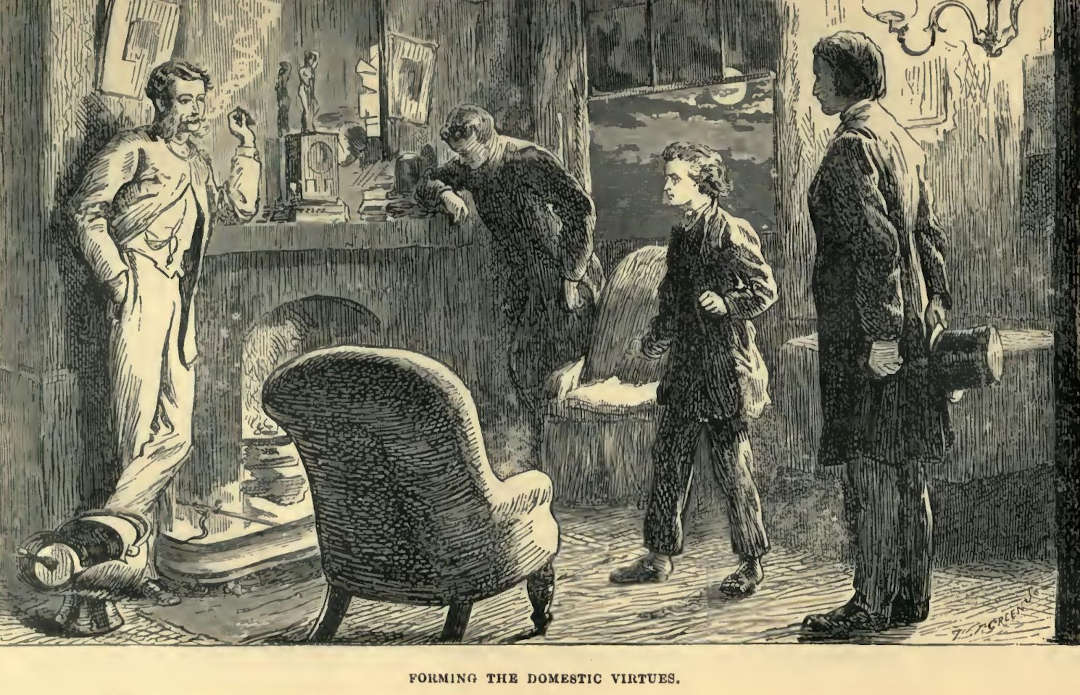
\includegraphics[scale=2.3]{02-06-01}

Composedly smoking, he leaned an elbow on the chimneypiece, at the side
of the fire, and looked at the schoolmaster. It was a cruel look, in its
cold disdain of him, as a creature of no worth. The schoolmaster looked
at him, and that, too, was a cruel look, though of the different kind,
that it had a raging jealousy and fiery wrath in it.

Very remarkably, neither Eugene Wrayburn nor Bradley Headstone looked at
all at the boy. Through the ensuing dialogue, those two, no matter
who spoke, or whom was addressed, looked at each other. There was some
secret, sure perception between them, which set them against one another
in all ways.

‘In some high respects, Mr Eugene Wrayburn,’ said Bradley, answering
him with pale and quivering lips, ‘the natural feelings of my pupils are
stronger than my teaching.’

‘In most respects, I dare say,’ replied Eugene, enjoying his cigar,
‘though whether high or low is of no importance. You have my name very
correctly. Pray what is yours?’

‘It cannot concern you much to know, but--’

‘True,’ interposed Eugene, striking sharply and cutting him short at his
mistake, ‘it does not concern me at all to know. I can say Schoolmaster,
which is a most respectable title. You are right, Schoolmaster.’

It was not the dullest part of this goad in its galling of Bradley
Headstone, that he had made it himself in a moment of incautious anger.
He tried to set his lips so as to prevent their quivering, but they
quivered fast.

‘Mr Eugene Wrayburn,’ said the boy, ‘I want a word with you. I have
wanted it so much, that we have looked out your address in the book, and
we have been to your office, and we have come from your office here.’

‘You have given yourself much trouble, Schoolmaster,’ observed
Eugene, blowing the feathery ash from his cigar. ‘I hope it may prove
remunerative.’

‘And I am glad to speak,’ pursued the boy, ‘in presence of Mr Lightwood,
because it was through Mr Lightwood that you ever saw my sister.’

For a mere moment, Wrayburn turned his eyes aside from the schoolmaster
to note the effect of the last word on Mortimer, who, standing on the
opposite side of the fire, as soon as the word was spoken, turned his
face towards the fire and looked down into it.

‘Similarly, it was through Mr Lightwood that you ever saw her again, for
you were with him on the night when my father was found, and so I found
you with her on the next day. Since then, you have seen my sister often.
You have seen my sister oftener and oftener. And I want to know why?’

‘Was this worth while, Schoolmaster?’ murmured Eugene, with the air of
a disinterested adviser. ‘So much trouble for nothing? You should know
best, but I think not.’

‘I don’t know, Mr Wrayburn,’ answered Bradley, with his passion rising,
‘why you address me--’

‘Don’t you? said Eugene. ‘Then I won’t.’

He said it so tauntingly in his perfect placidity, that the respectable
right-hand clutching the respectable hair-guard of the respectable watch
could have wound it round his throat and strangled him with it. Not
another word did Eugene deem it worth while to utter, but stood leaning
his head upon his hand, smoking, and looking imperturbably at the
chafing Bradley Headstone with his clutching right-hand, until Bradley
was wellnigh mad.

‘Mr Wrayburn,’ proceeded the boy, ‘we not only know this that I have
charged upon you, but we know more. It has not yet come to my sister’s
knowledge that we have found it out, but we have. We had a plan, Mr
Headstone and I, for my sister’s education, and for its being advised
and overlooked by Mr Headstone, who is a much more competent authority,
whatever you may pretend to think, as you smoke, than you could produce,
if you tried. Then, what do we find? What do we find, Mr Lightwood? Why,
we find that my sister is already being taught, without our knowing
it. We find that while my sister gives an unwilling and cold ear to our
schemes for her advantage--I, her brother, and Mr Headstone, the most
competent authority, as his certificates would easily prove, that could
be produced--she is wilfully and willingly profiting by other schemes.
Ay, and taking pains, too, for I know what such pains are. And so does
Mr Headstone! Well! Somebody pays for this, is a thought that naturally
occurs to us; who pays? We apply ourselves to find out, Mr Lightwood,
and we find that your friend, this Mr Eugene Wrayburn, here, pays. Then
I ask him what right has he to do it, and what does he mean by it, and
how comes he to be taking such a liberty without my consent, when I
am raising myself in the scale of society by my own exertions and Mr
Headstone’s aid, and have no right to have any darkness cast upon my
prospects, or any imputation upon my respectability, through my sister?’

The boyish weakness of this speech, combined with its great selfishness,
made it a poor one indeed. And yet Bradley Headstone, used to the little
audience of a school, and unused to the larger ways of men, showed a
kind of exultation in it.

‘Now I tell Mr Eugene Wrayburn,’ pursued the boy, forced into the use
of the third person by the hopelessness of addressing him in the first,
‘that I object to his having any acquaintance at all with my sister, and
that I request him to drop it altogether. He is not to take it into his
head that I am afraid of my sister’s caring for HIM--’

(As the boy sneered, the Master sneered, and Eugene blew off the
feathery ash again.)

--‘But I object to it, and that’s enough. I am more important to my
sister than he thinks. As I raise myself, I intend to raise her;
she knows that, and she has to look to me for her prospects. Now I
understand all this very well, and so does Mr Headstone. My sister is an
excellent girl, but she has some romantic notions; not about such things
as your Mr Eugene Wrayburns, but about the death of my father and other
matters of that sort. Mr Wrayburn encourages those notions to make
himself of importance, and so she thinks she ought to be grateful to
him, and perhaps even likes to be. Now I don’t choose her to be grateful
to him, or to be grateful to anybody but me, except Mr Headstone. And
I tell Mr Wrayburn that if he don’t take heed of what I say, it will be
worse for her. Let him turn that over in his memory, and make sure of
it. Worse for her!’

A pause ensued, in which the schoolmaster looked very awkward.

‘May I suggest, Schoolmaster,’ said Eugene, removing his fast-waning
cigar from his lips to glance at it, ‘that you can now take your pupil
away.’

‘And Mr Lightwood,’ added the boy, with a burning face, under the
flaming aggravation of getting no sort of answer or attention, ‘I hope
you’ll take notice of what I have said to your friend, and of what
your friend has heard me say, word by word, whatever he pretends to the
contrary. You are bound to take notice of it, Mr Lightwood, for, as I
have already mentioned, you first brought your friend into my sister’s
company, and but for you we never should have seen him. Lord knows none
of us ever wanted him, any more than any of us will ever miss him. Now
Mr Headstone, as Mr Eugene Wrayburn has been obliged to hear what I had
to say, and couldn’t help himself, and as I have said it out to the last
word, we have done all we wanted to do, and may go.’

‘Go down-stairs, and leave me a moment, Hexam,’ he returned. The boy
complying with an indignant look and as much noise as he could make,
swung out of the room; and Lightwood went to the window, and leaned
there, looking out.

‘You think me of no more value than the dirt under your feet,’ said
Bradley to Eugene, speaking in a carefully weighed and measured tone, or
he could not have spoken at all.

‘I assure you, Schoolmaster,’ replied Eugene, ‘I don’t think about you.’

‘That’s not true,’ returned the other; ‘you know better.’

‘That’s coarse,’ Eugene retorted; ‘but you DON’T know better.’

‘Mr Wrayburn, at least I know very well that it would be idle to set
myself against you in insolent words or overbearing manners. That lad
who has just gone out could put you to shame in half-a-dozen branches of
knowledge in half an hour, but you can throw him aside like an inferior.
You can do as much by me, I have no doubt, beforehand.’

‘Possibly,’ remarked Eugene.

‘But I am more than a lad,’ said Bradley, with his clutching hand, ‘and
I WILL be heard, sir.’

‘As a schoolmaster,’ said Eugene, ‘you are always being heard. That
ought to content you.’

‘But it does not content me,’ replied the other, white with passion. ‘Do
you suppose that a man, in forming himself for the duties I discharge,
and in watching and repressing himself daily to discharge them well,
dismisses a man’s nature?’

‘I suppose you,’ said Eugene, ‘judging from what I see as I look at you,
to be rather too passionate for a good schoolmaster.’ As he spoke, he
tossed away the end of his cigar.

‘Passionate with you, sir, I admit I am. Passionate with you, sir, I
respect myself for being. But I have not Devils for my pupils.’

‘For your Teachers, I should rather say,’ replied Eugene.

‘Mr Wrayburn.’

‘Schoolmaster.’

‘Sir, my name is Bradley Headstone.’

‘As you justly said, my good sir, your name cannot concern me. Now, what
more?’

‘This more. Oh, what a misfortune is mine,’ cried Bradley, breaking off
to wipe the starting perspiration from his face as he shook from head to
foot, ‘that I cannot so control myself as to appear a stronger creature
than this, when a man who has not felt in all his life what I have felt
in a day can so command himself!’ He said it in a very agony, and even
followed it with an errant motion of his hands as if he could have torn
himself.

Eugene Wrayburn looked on at him, as if he found him beginning to be
rather an entertaining study.

‘Mr Wrayburn, I desire to say something to you on my own part.’

‘Come, come, Schoolmaster,’ returned Eugene, with a languid approach to
impatience as the other again struggled with himself; ‘say what you have
to say. And let me remind you that the door is standing open, and your
young friend waiting for you on the stairs.’

‘When I accompanied that youth here, sir, I did so with the purpose of
adding, as a man whom you should not be permitted to put aside, in case
you put him aside as a boy, that his instinct is correct and right.’
Thus Bradley Headstone, with great effort and difficulty.

‘Is that all?’ asked Eugene.

‘No, sir,’ said the other, flushed and fierce. ‘I strongly support him
in his disapproval of your visits to his sister, and in his objection to
your officiousness--and worse--in what you have taken upon yourself to
do for her.’

‘Is THAT all?’ asked Eugene.

‘No, sir. I determined to tell you that you are not justified in these
proceedings, and that they are injurious to his sister.’

‘Are you her schoolmaster as well as her brother’s?--Or perhaps you
would like to be?’ said Eugene.

It was a stab that the blood followed, in its rush to Bradley
Headstone’s face, as swiftly as if it had been dealt with a dagger.
‘What do you mean by that?’ was as much as he could utter.

‘A natural ambition enough,’ said Eugene, coolly. ‘Far be it from me
to say otherwise. The sister who is something too much upon your lips,
perhaps--is so very different from all the associations to which she had
been used, and from all the low obscure people about her, that it is a
very natural ambition.’

‘Do you throw my obscurity in my teeth, Mr Wrayburn?’

‘That can hardly be, for I know nothing concerning it, Schoolmaster, and
seek to know nothing.’

‘You reproach me with my origin,’ said Bradley Headstone; ‘you cast
insinuations at my bringing-up. But I tell you, sir, I have worked my
way onward, out of both and in spite of both, and have a right to be
considered a better man than you, with better reasons for being proud.’

‘How I can reproach you with what is not within my knowledge, or how
I can cast stones that were never in my hand, is a problem for the
ingenuity of a schoolmaster to prove,’ returned Eugene. ‘Is THAT all?’

‘No, sir. If you suppose that boy--’

‘Who really will be tired of waiting,’ said Eugene, politely.

‘If you suppose that boy to be friendless, Mr Wrayburn, you deceive
yourself. I am his friend, and you shall find me so.’

‘And you will find HIM on the stairs,’ remarked Eugene.

‘You may have promised yourself, sir, that you could do what you
chose here, because you had to deal with a mere boy, inexperienced,
friendless, and unassisted. But I give you warning that this mean
calculation is wrong. You have to do with a man also. You have to do
with me. I will support him, and, if need be, require reparation for
him. My hand and heart are in this cause, and are open to him.’

‘And--quite a coincidence--the door is open,’ remarked Eugene.

‘I scorn your shifty evasions, and I scorn you,’ said the schoolmaster.
‘In the meanness of your nature you revile me with the meanness of my
birth. I hold you in contempt for it. But if you don’t profit by this
visit, and act accordingly, you will find me as bitterly in earnest
against you as I could be if I deemed you worth a second thought on my
own account.’

With a consciously bad grace and stiff manner, as Wrayburn looked so
easily and calmly on, he went out with these words, and the heavy door
closed like a furnace-door upon his red and white heats of rage.

‘A curious monomaniac,’ said Eugene. ‘The man seems to believe that
everybody was acquainted with his mother!’

Mortimer Lightwood being still at the window, to which he had in
delicacy withdrawn, Eugene called to him, and he fell to slowly pacing
the room.

‘My dear fellow,’ said Eugene, as he lighted another cigar, ‘I fear my
unexpected visitors have been troublesome. If as a set-off (excuse the
legal phrase from a barrister-at-law) you would like to ask Tippins to
tea, I pledge myself to make love to her.’

‘Eugene, Eugene, Eugene,’ replied Mortimer, still pacing the room, ‘I am
sorry for this. And to think that I have been so blind!’

‘How blind, dear boy?’ inquired his unmoved friend.

‘What were your words that night at the river-side public-house?’ said
Lightwood, stopping. ‘What was it that you asked me? Did I feel like a
dark combination of traitor and pickpocket when I thought of that girl?’

‘I seem to remember the expression,’ said Eugene.

‘How do YOU feel when you think of her just now?’

His friend made no direct reply, but observed, after a few whiffs of his
cigar, ‘Don’t mistake the situation. There is no better girl in all this
London than Lizzie Hexam. There is no better among my people at home; no
better among your people.’

‘Granted. What follows?’

‘There,’ said Eugene, looking after him dubiously as he paced away to
the other end of the room, ‘you put me again upon guessing the riddle
that I have given up.’

‘Eugene, do you design to capture and desert this girl?’

‘My dear fellow, no.’

‘Do you design to marry her?’

‘My dear fellow, no.’

‘Do you design to pursue her?’

‘My dear fellow, I don’t design anything. I have no design whatever.
I am incapable of designs. If I conceived a design, I should speedily
abandon it, exhausted by the operation.’

‘Oh Eugene, Eugene!’

‘My dear Mortimer, not that tone of melancholy reproach, I entreat. What
can I do more than tell you all I know, and acknowledge my ignorance
of all I don’t know! How does that little old song go, which, under
pretence of being cheerful, is by far the most lugubrious I ever heard
in my life?

\begin{verbatim}
     "Away with melancholy,
     Nor doleful changes ring
     On life and human folly,
     But merrily merrily sing
                              Fal la!”
\end{verbatim}

Don’t let us sing Fal la, my dear Mortimer (which is comparatively
unmeaning), but let us sing that we give up guessing the riddle
altogether.’

‘Are you in communication with this girl, Eugene, and is what these
people say true?’

‘I concede both admissions to my honourable and learned friend.’

‘Then what is to come of it? What are you doing? Where are you going?’

‘My dear Mortimer, one would think the schoolmaster had left behind him
a catechizing infection. You are ruffled by the want of another cigar.
Take one of these, I entreat. Light it at mine, which is in perfect
order. So! Now do me the justice to observe that I am doing all I can
towards self-improvement, and that you have a light thrown on those
household implements which, when you only saw them as in a glass darkly,
you were hastily--I must say hastily--inclined to depreciate. Sensible
of my deficiencies, I have surrounded myself with moral influences
expressly meant to promote the formation of the domestic virtues.
To those influences, and to the improving society of my friend from
boyhood, commend me with your best wishes.’

‘Ah, Eugene!’ said Lightwood, affectionately, now standing near him,
so that they both stood in one little cloud of smoke; ‘I would that you
answered my three questions! What is to come of it? What are you doing?
Where are you going?’

‘And my dear Mortimer,’ returned Eugene, lightly fanning away the smoke
with his hand for the better exposition of his frankness of face and
manner, ‘believe me, I would answer them instantly if I could. But
to enable me to do so, I must first have found out the troublesome
conundrum long abandoned. Here it is. Eugene Wrayburn.’ Tapping his
forehead and breast. ‘Riddle-me, riddle-me-ree, perhaps you can’t tell
me what this may be?--No, upon my life I can’t. I give it up!’



